\documentclass[tikz,10pt]{standalone}

%%%%%%%%%%%%%%%%%%%%%%%%%%%%%%%%%%%%%%%%%
%                                       %
%                MY COLORS              %
%                                       %
%%%%%%%%%%%%%%%%%%%%%%%%%%%%%%%%%%%%%%%%%
 \definecolor{ccred}{cmyk}{0, 0.87, 0.8, 0.21}
 \definecolor{cccitrouille}{RGB}{223,109,20}
 \definecolor{cccanard}{RGB}{4,139,154}
 \definecolor{ccorangebrule}{RGB}{204,85,0}
 \definecolor{ccargile}{RGB}{239,239,239}
 %%%%%%%%%%%%%%%%%%%%%%%%%%%%%%%%%%%%%%%%%

\begin{document}
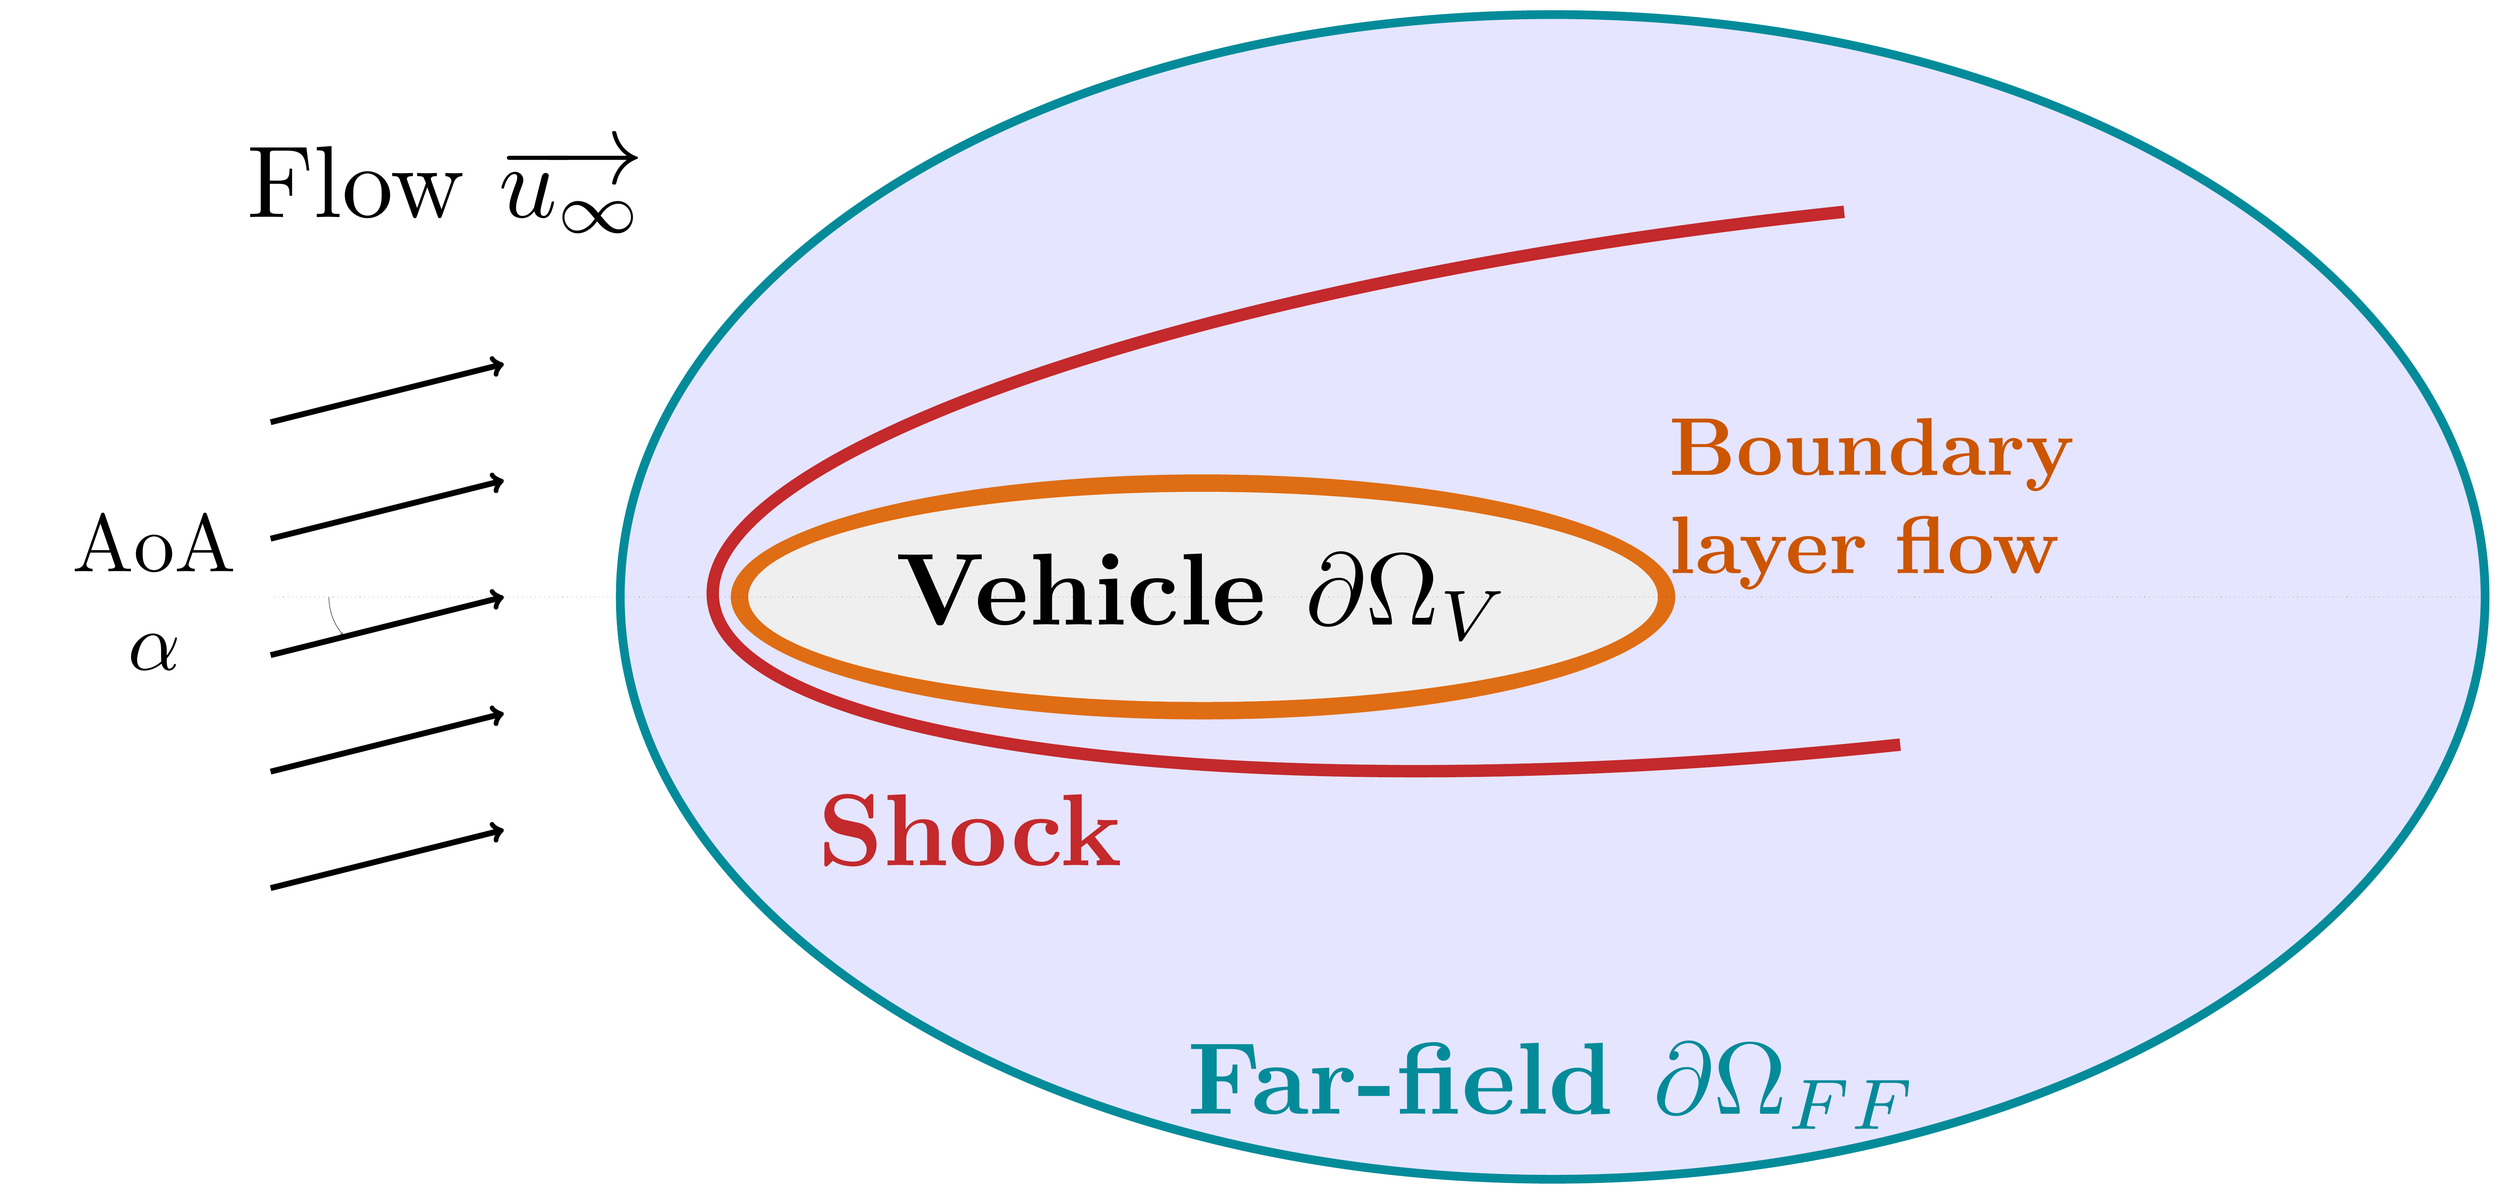
\begin{tikzpicture}[scale=4]

  % Flow
  \draw[fill=white!90!blue] (6,0) circle [x radius=8cm, y radius=5cm];

  % Boundary layer flow
  \draw[fill=cccitrouille, color=cccitrouille] (3,0) circle [x radius=4.05cm, y radius=1.05cm];

  % Choc
  \draw[line width=4.25mm, ccred, rotate=6] (8.8,2.4) arc [start angle=90, end angle=270, x radius=10cm, y radius=2.3cm];

  % Vehicle
  \draw[fill=white, color=white] (3,0) circle [x radius=3.9cm, y radius=0.9cm];
  \filldraw[fill=ccargile, color=ccargile] (3,0) circle [x radius=3.9cm, y radius=0.9cm];

  % Farfield
  \draw[line width=3mm, cccanard] (6,0) circle [x radius=8cm, y radius=5cm];

  % Amont
  \draw[->, line width=2mm] (-5,-2.5) -- (-3,-2);
  \draw[->, line width=2mm] (-5,-1.5) -- (-3,-1);
  \draw[->, line width=2mm] (-5,-0.5) -- (-3,0);
  \draw[->, line width=2mm] (-5,0.5) -- (-3,1);
  \draw[->, line width=2mm] (-5,1.5) -- (-3,2);
  

  % Axis
  \draw (-5,0) node (begin) {};
  \draw (14,0) node (end) {};
  \draw[loosely dotted] (begin) -- (end) ;

  % AoA (Angle of Attack)
  \draw (-5,-0.5) node (u1) {};
  \draw (-3, 0) node (u2) {};
  \draw[->] (-4.5,0) arc (180:220:0.5cm);
 
 % Légende en anglais
 \draw(9,0.8) node[scale=8, color=ccorangebrule, text width=2cm] (cl) {\textbf{Boundary layer flow}};
 \draw(-3.5,3.5) node[scale=10, black] (ecoulement) {Flow $\overrightarrow{u_\infty}$};
 \draw(3,0) node[scale=10] (objet) {\textbf{Vehicle $\partial \Omega_V$}};
 \draw(1,-2.0) node[scale=10, ccred] (choc) {\textbf{Shock}};
 \draw(6,-4.2) node[scale=10, cccanard] (amont) {\textbf{Far-field $\partial \Omega_{FF}$}};
 \draw(-6,0.5) node[scale=8, black, text width=1cm] (AoA) {\begin{center} AoA $\alpha$ \end{center}};
 
 % Legend translated in french
 %\draw(10,0.8) node[scale=8, color=ccorangebrule, text width=3cm] (cl) {\begin{center} \textbf{Couche limite fluide} \end{center}};
 %\draw(-3.5,3.8) node[scale=10, black, text width=2.5cm] (ecoulement) {\begin{center} Vitesse amont $\overrightarrow{u_\infty}$ \end{center}};
 %\draw(3,0) node[scale=10] (objet) {\textbf{Véhicule}};
 %\draw(1,-2.0) node[scale=10, ccred] (choc) {\textbf{Choc}};
 %\draw(6,-4) node[scale=10, cccanard] (amont) {\textbf{Frontière externe}};
 %\draw(-6,0.5) node[scale=8, black, text width=0.5cm] (AoA) {\begin{center} AA $\alpha$ \end{center}};

\end{tikzpicture}
\end{document}